\documentclass{article}

\usepackage{a4wide}
\usepackage[utf8]{inputenc}
\usepackage[T1]{fontenc}
\usepackage[french]{babel}
\usepackage[babel=true]{csquotes} % guillemets français
\usepackage{graphicx}
\graphicspath{{Images/}}
\usepackage{color}
\usepackage{hyperref}
\hypersetup{colorlinks,linkcolor=,urlcolor=blue}

\usepackage{amsmath}
\usepackage{amssymb}


\title{\textbf{ Rapport - Developpement Mobile \\ Démineur}}
\author{Kamarouzamane Combo, Jeremie Legros\\
		L3 informatique\\
	  }
\date{\today}

\begin{document}

\maketitle % pour écrire le titre


%% Résumé:
\begin{abstract}
	Dans ce rapport, nous allons vous présenter ce que nous avons pu voire dans l'UE Développement pour Mobile, et le projet que l'on a fait cette année.  Nous avons choisie de nous inspirer du jeu Démineur et d'en faire une version Android et iOS. Nous vous exposons ici le principe du jeu, le fonctionnement de l'application et son développement.\\

	\textbf{Mots clés }: Android Studio, Xcode, Java, Swift, Activity
\end{abstract}


\section{Introduction}
\label{section:intro} % pour faire référence à la section ailleurs (\ref{...} voir plus bas)
	Dans le cadre de l' UE Développement pour Mobile, nous avons décidé de réaliser une version simple du jeu Démineur.
Il nous était demandé de réaliser le même jeu sur les deux plateformes ( Android et iOS.~\cite{statOS} ). 
La version Android est programmé en Jave et celle iOS est programmé en Swift. Pour commancer, nous vous présenterons d'abord quel type de jeu nous avons voulu développer, puis nous explorerons l' architecture du code.


\section{Description générale de l'application}

\textbf {Comment jouer au Démineur ?}\\
Vous devez déminer ce champ de mines. Pour cela, il a été découpé en carrés, qui peuvent contenir soit une seule mine Mine Démineur, soit aucune. Au début, les mines, enterrées, ne sont évidement pas visibles.Pour gagner au Démineur, il vous faut déterminer l'emplacement de toutes les mines. Pour atteindre cet objectif, vous pourrez prendre connaissance du nombre de mines (\textbf{1,2,3 ou 4}) dans le voisinage immédiat d'une case, en appuyant sur celle-ci et à condition qu'elle soit vide. Si jamais vous appuyez sur une case contenant une mine, celle-ci explose (\textbf{B}) Explosion Démineur et vous perdez. Il est possible de planter un drapeau (en utilisant le \textbf{bouton switch}) pour marquer l'emplacement supposé d'une mine, Si la case appuyée est vide, toutes les cases vides adjacentes s'ouvriront recursivement.\\
Pour gagner, il ne doit pas y avoir de mines incorrectement marquées avec un drapeau. Par contre, il n'est pas nécessaire de marquer toutes les mines pour terminer; vous avez juste besoin de déterminer toutes les cases vides.\\
\begin{center}
   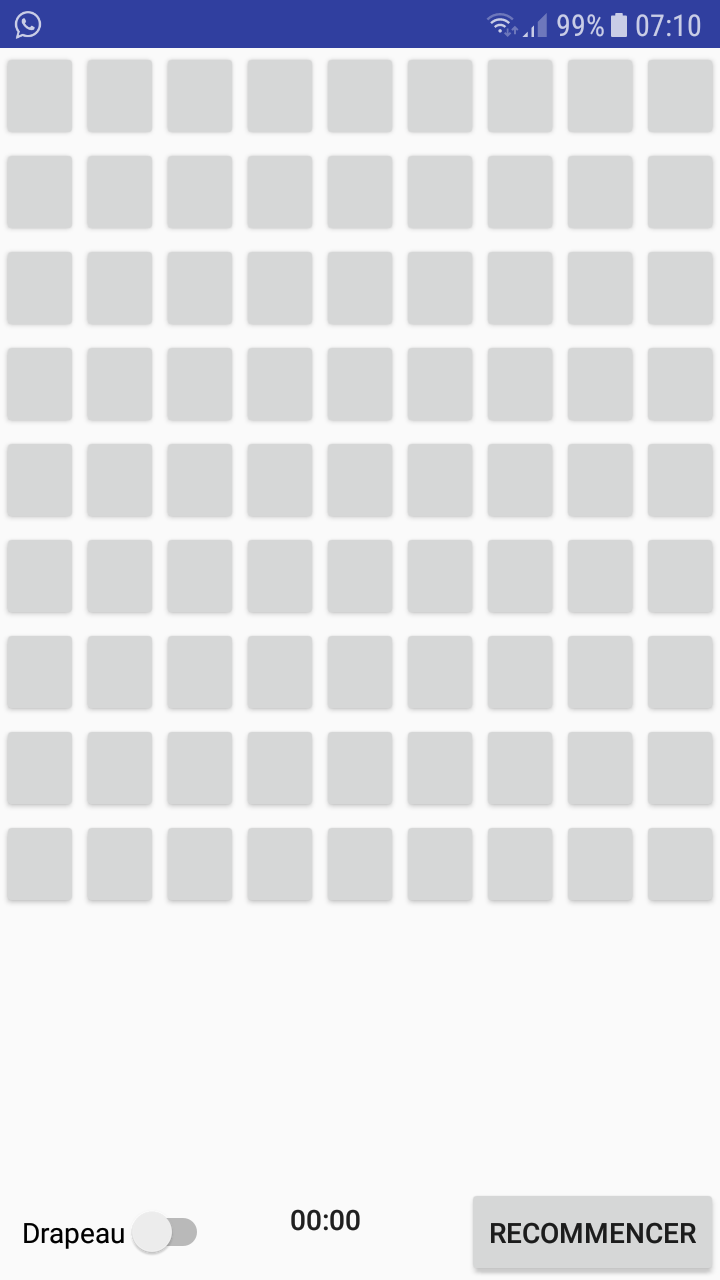
\includegraphics[scale=0.12]{1.png}
   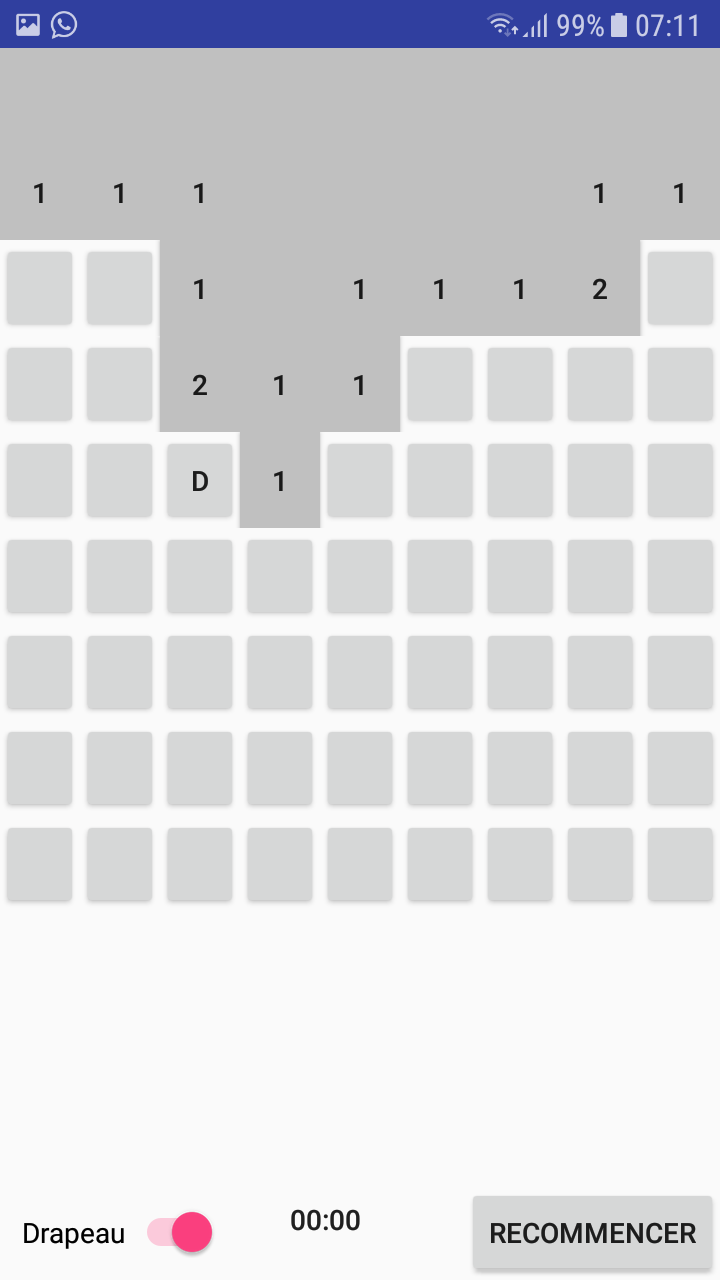
\includegraphics[scale=0.12]{2.png}
   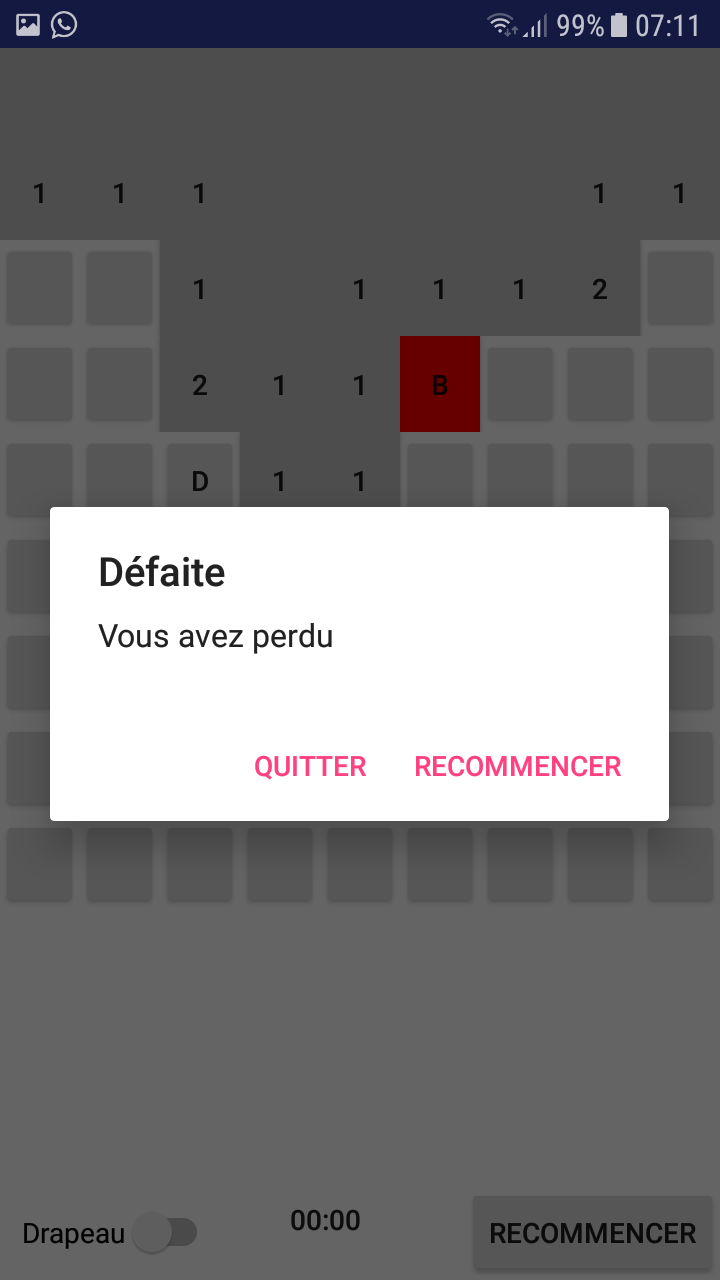
\includegraphics[scale=0.12]{3.png}
\end{center}

\textbf {Mais que fait-elle exactement ?} \\
	Au lancement de l’ application, la page d’ accueil apparaître et donner la
possibilité à l' utilisateur de jouer une nouvelle partie (choix : le niveau de difficulté), de reprendre une partie sauvegardée ou de consulter la liste des scores enregistrés.

Voici une capture d'écran du Main Activity:
\begin{center}
  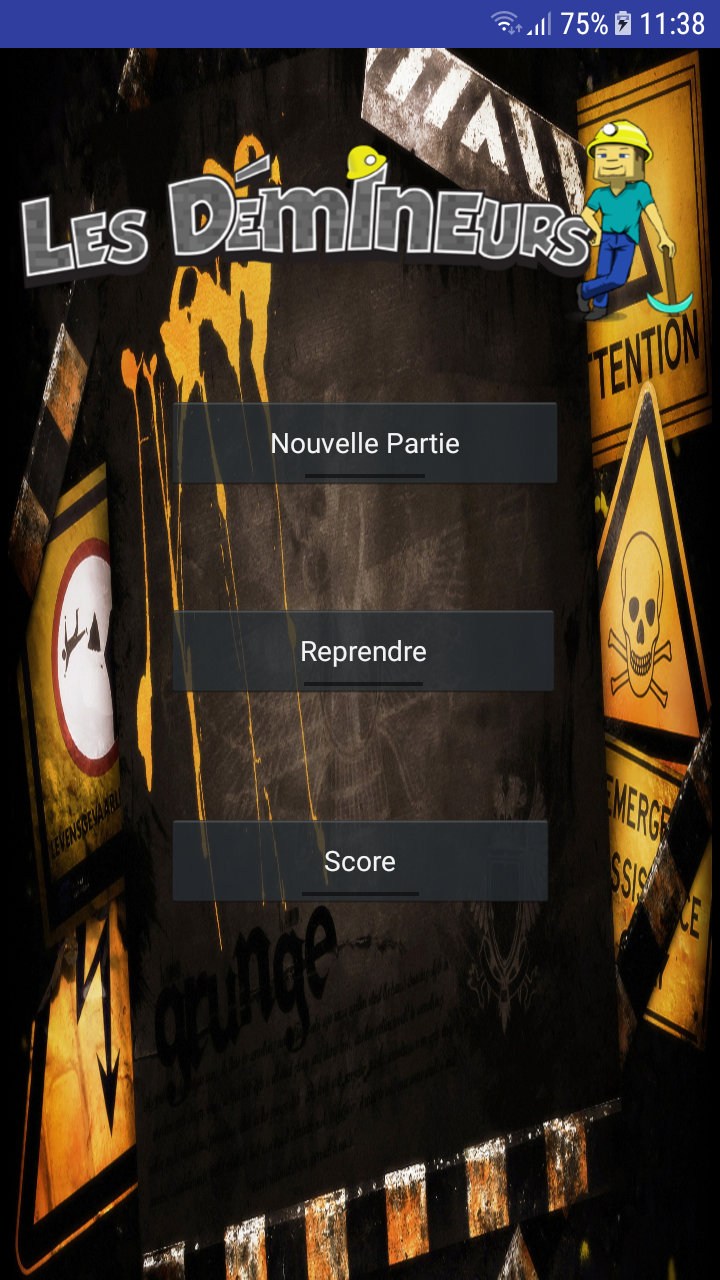
\includegraphics[scale=0.12]{Main.png}
\end{center}

Avant que l'utilisateur puisse choisir le niveau de difficulté, on a mis en place une activity 
de présentation du jeu et des règles du jeu. En suite il saisir la difficulté, toute fois s'il veux
accéder au jeu sans  avoir saisie de difficulté au préalable, il s'affichera un message d' erreur 
qui lui demandera de choisir un niveau de difficulté. \\
 
\begin{center}
  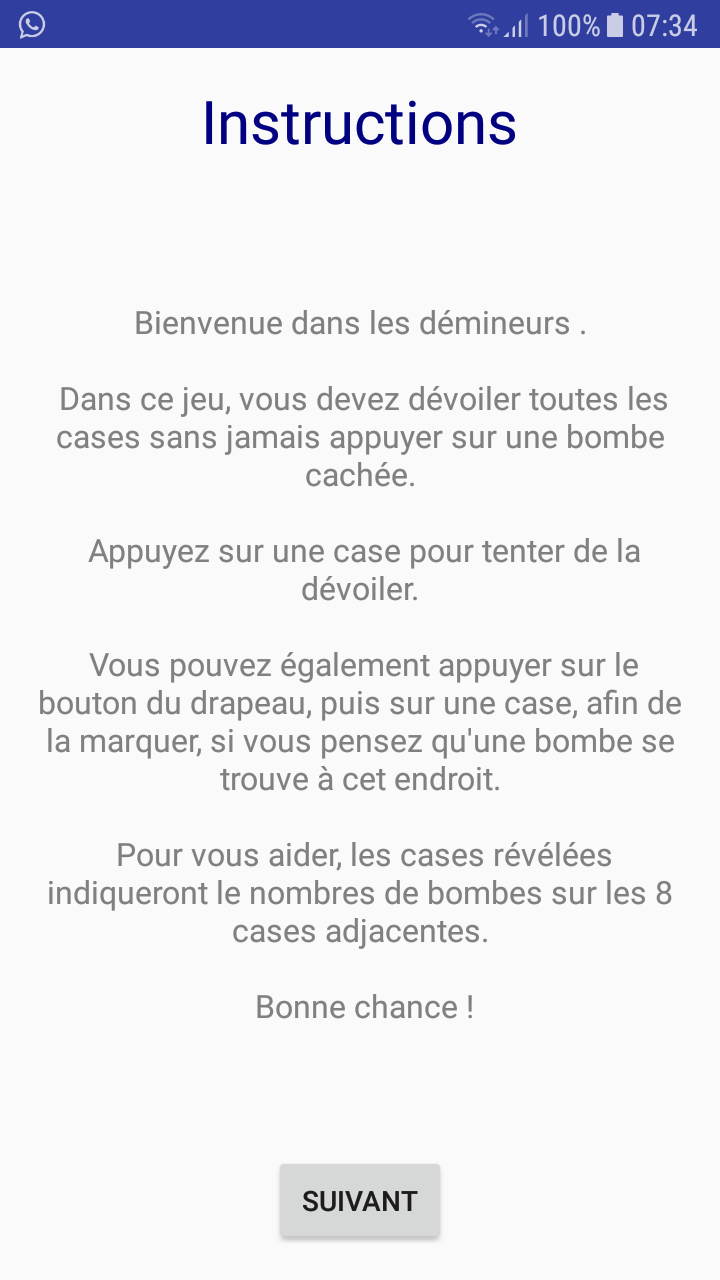
\includegraphics[scale=0.12]{Intro.png}
  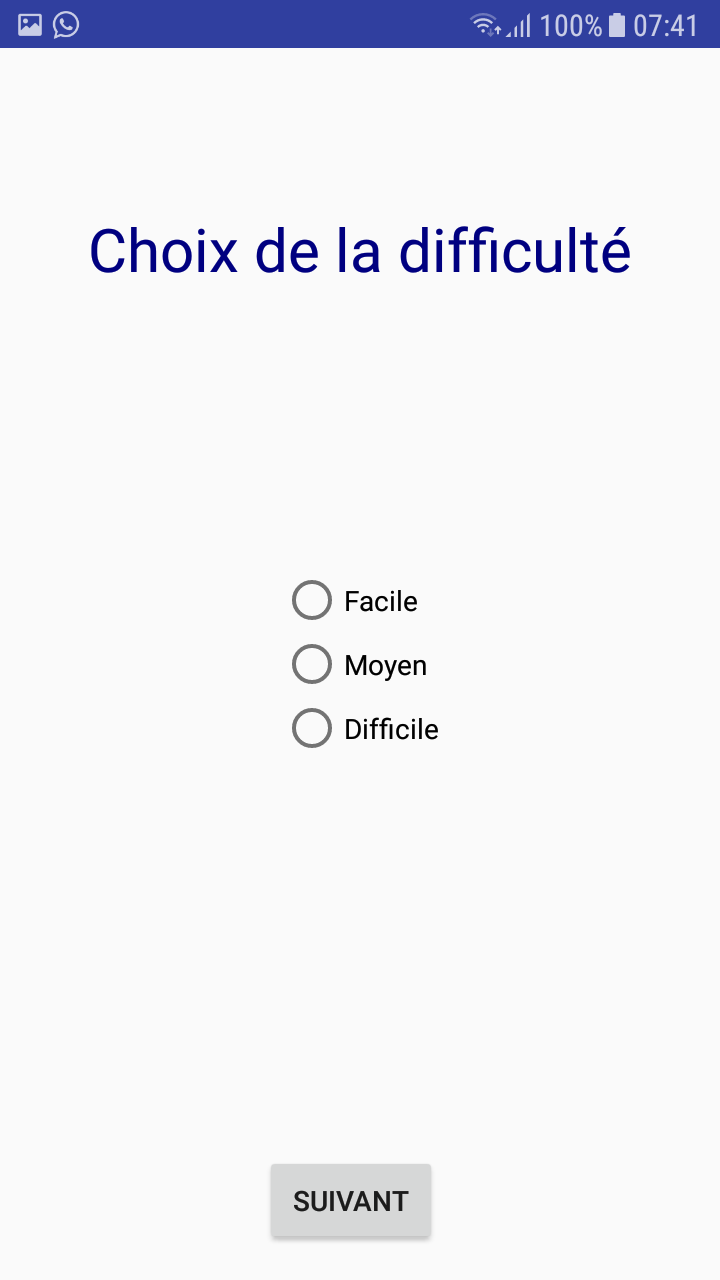
\includegraphics[scale=0.12]{Difficulte.png}
\end{center}

L' application est jouable sur \textit{Android}~\cite{androidDoc} et iOS \textit{iOS}~\cite{iosDoc}, elle fonctionne correctement sur tout type d' \'ecran (grand, petit, …), en mode portrait et paysage.\\




% \cite{...} permet de faire référence à des éléments de la
% bibliographie.

\section{Architecture du code}
% \ref{...} permet de faire référence à un élément défini
% ailleurs dans le document (voir \label{...} plus haut).
\subsection{Accueil et activityaccueil.xml}
L’écran d’accueil affiche le titre du jeu et comporte trois boutons, l’un pour lancer une nouvelle
partie et le second pour accéder à la liste des partie en cours  enregistrés, et la dernière pour accéder à la liste des scores enregistrés. Lorsqu’on appuie sur le premier, on est dirigé vers l’activité d' indtroduction, tandis que les autres nous envoie sur des activités
gérant et parties en cours et les scores.

\subsection{Android} %% une sous-section
Pour écrire du code, on peut par exemple utiliser l'environnement
\textit{verbatim}:
\begin{verbatim}
public class Main {
   public static void main(String[] args) {
      System.out.println("Hello World!");
   }
}
\end{verbatim}

\subsection{iOS} %% une autre sous-section


\section{Quelques points délicats/intéressants}


\section{Conclusion générale}
	Cette projet était une bonne expérience, et qui plus était enrichissante.
Grâce elle, elle nous a permis de pouvoir développer des applications sur les deux système,
Android et iOS, de créer plusieurs projets,cette UE nous permis de pouvoir travailler en autonomie
et de ce fait, effectuer nos propres recherches, tester de nouvelles choses, faire des erreurs, et en
apprendre davantage grâce à elles.


%%% La bibliographie:
\bibliographystyle{plain}
\bibliography{ma_biblio}

\end{document}
